\documentclass[11pt, a4paper]{article}
\usepackage{natbib}
\usepackage{eso-pic}
\usepackage{amsmath} % flere matematikkommandoer
\usepackage{amssymb}
\usepackage[utf8]{inputenc} % æøå
\usepackage[T1]{fontenc} % mere æøå
\usepackage[danish, english]{babel} % orddeling
\usepackage{verbatim} % så man kan skrive ren tekst
\usepackage{listings}
\usepackage{graphicx}
\usepackage{booktabs}
\usepackage{enumitem}
\usepackage{placeins}
\usepackage[colorlinks=false]{hyperref}
\usepackage{tocbibind}
\usepackage{fancyvrb}
\usepackage{framed}

% Default fixed font does not support bold face
\DeclareFixedFont{\ttb}{T1}{txtt}{bx}{n}{10} % for bold
\DeclareFixedFont{\ttm}{T1}{txtt}{m}{n}{10}  % for normal

% Custom colors
\usepackage{color}
\definecolor{deepblue}{rgb}{0,0,0.5}
\definecolor{deepred}{rgb}{0.6,0,0}
\definecolor{deepgreen}{rgb}{0,0.5,0}

% Python style for highlighting
\newcommand\pythonstyle{\lstset{
        language=Python,
        basicstyle=\ttm,
        otherkeywords={self},             % Add keywords here
        keywordstyle=\ttb\color{deepblue},
        emph={MyClass,__init__},          % Custom highlighting
        emphstyle=\ttb\color{deepred},    % Custom highlighting style
        stringstyle=\color{deepgreen},
        frame=tb,                         % Any extra options here
        showstringspaces=false            %
    }}


% Python environment
\lstnewenvironment{python}[1][]
{
    \pythonstyle
    \lstset{#1}
}
{}

% Python for external files
\newcommand\pythonexternal[2][]{{
        \pythonstyle
        \lstinputlisting[#1]{#2}}}

% Python for inline
\newcommand\pythoninline[1]{{\pythonstyle\lstinline!#1!}}

\title{
  \vspace{3cm}
  \Huge{Projektkursus i Systemudvikling} \\[.10cm]
  \Large{PoP-Webhelp}
}

\author{
    Christian Kjær Larsen \texttt{(011292)} \\[.4cm]
    Lukas Svarre Engedal \texttt{(210790)} \\[.4cm]
    Tobias Sønderskov Hansen \texttt{(240395)} \\[.4cm]
    Instruktor: Aske Mottelson\\[.4cm]
    \vspace{9cm}
}

\begin{document}
\selectlanguage{danish}
\AddToShipoutPicture*{\put(0,0){\includegraphics*[viewport=0 0 700 600]{includes/nat-farve}}}
\AddToShipoutPicture*{\put(0,602){\includegraphics*[viewport=0 600 700 1600]{includes/nat-farve}}}

%% Change `ku-en` to `nat-en` to use the `Faculty of Science` header
\AddToShipoutPicture*{\put(0,0){\includegraphics*{includes/nat-en}}}

\clearpage\maketitle
\thispagestyle{empty}

\newpage

\selectlanguage{english}
\begin{abstract}
This report presents the development of an e-learning system for use in the newly created introductory computer science course at the Department of Computer Science at University of Copenhagen, called \emph{Programmering og Problemløsning}(Programming and Problemsolving). The clients are Martin Dybdal and Oleksandr Shturmov, both employed at the department, who will be responsible for the course. In the course, the students will be taught the programming language \verb!F#!.

The aim of the e-learning system is to introduce new students to programming in a simple and user-friendly way, and to teach them various basic ideas and concepts in programming in general, and \verb!F#! in particular. This is done by presenting the students with a series of different exercises, sorted based on subject and difficulty, and presented to students in a specific and meaningful order. The students can also get hints to the exercises if needed.

Another important part is the administration of the system, which includes managing the exercises and supervising how well the students are doing. The admins should be able to easily delete or modify existing exercises as well as adding new ones. They should also be able to get various statistics about how the students are doing in order to improve and optimize the exercises.
\end{abstract}
\selectlanguage{danish}
\newpage

\section*{Indholdsfortegnelse}
\label{sec:toc}
\makeatletter
\@starttoc{toc}
\makeatother

\thispagestyle{empty}
\newpage

\pagestyle{plain}
\setcounter{page}{1}
\pagenumbering{arabic}

\section{Review}
\label{sec:review}

\subsection{Programming as theory building}
\label{sub:programming_as_theory_building}
Artiklen beskriver en måde at betragte programmering på, kaldet \emph{Theory Building View}, hvor fokus er på teorien og menneskerne bag et program, snarere end på selve programmet og koden.

Artiklen starter med et par eksempler på situationer hvor et projekt er udviklet af ét hold af programmører, men vedligeholdt og viderebygget af et andet hold. Der argumenteres så for at uanset hvor omfattende og detaljeret dokumentation det oprindelige hold af udviklere har produceret, vil det hold der senere tager over aldrig fuldstændig kunne overtage og videreføre projektet uden tab af effektivitet og sammenhæng. Dette kan dog mindskes eller måske endda helt undgås ved at det nye hold er i tæt kontakt med det oprindelige hold af udviklere og kan trække på, og nyde godt af, deres oprindelige idéer og erfaringer med projektet.

Artiklen definerer det at have en teori om et program sådan at hvis en person har en teori om et bestemt program betyder det at personen har en omfattende viden om ikke bare hvordan programmet virker helt konkret, men også hvordan det er forbundet og interagerer med den virkelige verden. Personen er derfor i stand til både at forklare, forsvare og diskutere hvordan programmet opfører sig i forskellige situationer og på forskellige tidspunkter. Og det er netop denne form for viden der argumenteres for ikke bare kan videregives i form af dokumentation og regler, men som skal tilegnes ved selv at få erfaring med programmet, samt i høj grad også ved at interagere med og lære af andre med denne viden.

Artiklen forklarer at der hvor \emph{the Theory Building View} virkelig adskiller sig fra et mere traditionelt syn på programmering er når det kommer til ændringer og udvidelser af programmer. Hvis man ser på det meget simpelt er et program i virkeligheden bare en række af filer indeholdende tekst, med en tilhørende række af tekstfiler der beskriver denne tekst i form af dokumentation. Man kunne derfor fristes til at tro at det burde være meget simpelt at ændre og tilføje til denne tekst, og derfor også forvente at ændringer og tilføjelser til programmer er simple og billige.

Hvis man antager \emph{the Theory Building View} er situationen dog en helt anden; her svarer en ændring af programmet til en ændring af selve teorien bag programmet, og det er langt mere avanceret. For at kunne ændre i, og tilføje til, teorien bag et program på en effektiv og meningsfuld måde kræver det, at man har en grundlæggende forståelse af teorien, og artiklen går endda så langt som til at hævde, at hvis det ikke er tilfældet, så er ændringer så godt som umulige. Det forklares at det ofte er dette der fører til at programmer 'dør ud', og at det i sådanne situationer nogen gange faktisk kan være den bedste idé at lade det ske og så i stedet lade programmet 'genopstå' ved at lade et nyt hold af programmører danne en ny teori.

Overordnet set passer \emph{the Theory Building View} meget godt sammen med de ting vi lærer i PKSU-kurset og læser i OOSE\cite{OOSE} bogen. Vi har lært meget om, og haft meget fokus på, at lave en masse arbejde allerede inden vi går i gang med at 'programmere', altså med at skrive selve koden. Vi bruger tid på at lave grundige analyser af vores problem- og anvendelsesområde, vi arbejder med kravene til systemet, vi laver design af vores system og vores objekter, vi laver use cases og diverse andre grafer der beskriver vores system, vi laver forskellige og grundige former for tests osv. Alt dette kan jo meget vel ses som at vi opbygger en teori omkring vores system, idet at vi dermed tilegner os den viden der skal til for at kunne forklare, forsvare og argumentere for hvorfor vores system virker som det gør og hvordan det er forbundet med den virkelige verden, hvilket jo netop er sådan som en teori blev defineret i artiklen.

Enhver der har arbejdet med et program skrevet af en anden ved også at selvom man læser både koden og dokumentationen grundigt, så er det ikke altid helt nemt at forstå fuldstændig hvad der sker og hvorfor, og at skulle ændre i, eller tilføje til, koden kan være noget af en opgave. Hvis man derimod kan snakke med én af dem der har været med til at udvikle programmet, og som dermed har styr på teorien bag, og kan stille spørgsmål og få forklaret ting man ikke helt forstår, så gør det det væsentlig nemmere.

Endelig kan man jo som datalog ikke være andet end enig i det syn på programmører som \emph{the Theory Building View} er fortaler for; nemlig at programmører ikke bare er komponenter i en industriel produktion som man bare kan smide væk og erstatte efter lyst og behov, men at de derimod er en vigtig og integral del af ethvert it-system, og fortjener den dertilhørende respekt og status.

\subsection{Extreme Programming}
\label{sub:extreme_programming}
Artiklen diskuterer nogle af de problemer der er ved moderne softwareudvikling, med fokus på hvordan Extreme Programming metodologien håndterer disse udfordringer. Artiklen adresserer det den beskriver som de to væsentligste udfordringer inden for softwareudvikling:
\begin{itemize}
\item Hurtig levering af software
\item Følge med i nærmest konstant forandring
\end{itemize}
Specielt de mere traditionelle og \emph{tungere} fremgangsmåder har svært ved at håndtere de hyppige ændringer som markedet kræver, hvorimod Extreme Programming (XP) er en metodologi opbygget netop omkring dette.

En tendens inden for softwareudvikling er at strukturere systemet med øje for funktionalitet der \emph{muligvis} skal implementeres senere og derved spare fremtidigt arbejde, såkaldt \emph{anticipatory design}. Dette fraråder XP dog, til fordel for en fremgangsmåde hvor der kun laves hvad der skal bruges i øjeblikket, uden at lade sig hæmme af spekulation om fremtidig funktionalitet.

Ligesom med andre agile metoder foregår udviklingen i korte iterationer, i tilfældet for XP varer disse iterationer som udgangspunkt 3 uger. 

Et andet grundlæggende princip siger at hver udgivelse skal være så lille som mulig. En fordel ved dette er at det giver hyppigere og mere relevant feedback, der så kan bruges i den efterfølgende udvikling.

En ting der særligt kendetegner XP er dets fokus på refaktorering. En kendt problematik er programkodes tendens til af forskellige grunde at forværres med tiden, og med hyppige ændringer sker denne proces blot endnu hurtigere. XP forsøger at løse dette problem ved at have refaktorering som en central del af processen. I praksis sker dette ved, at når ny funktionalitet skal tilføjes gøres det så simpelt som muligt, hvilket ofte vil involvere refaktorering af dele af koden.

Extreme Programming omfatter en forholdsvis lang række principper og værktøjer, om det er anvendeligt afhænger dog af det pågældende projekt, man kan generelt se metoden som en række retningslinjer og må så vurdere hvad der er relevant for situationen. Særligt er antallet af deltagere i et udviklingsprojekt afgørende for hvilken udviklingsmetode der er bedst egnet. Forholdsvis \emph{lette} metoder som XP er specielt egnet til mindre grupper på omkring 10 personer, hvor kommunikation let kan klares ansigt til ansigt mellem udviklerne. I større projekter med eksempelvis flere hundrede udviklere er kommunikationen dog mere kompliceret, og der vil da være større brug for at koordinere kommunikationen, hvilket kan gøre at andre metoder vil være mere hensigtsmæssige.

Oplagt kan artiklen perpsektivere til udviklingsmetoden præsenteret i artiklen \emph{The M.A.D. Experience} fra forrige delaflevering. På trods af at begge metoder gør brug af en agil fremgangsmåde er der alligevel nogle interessante forskelle mellem dem, særligt med hensyn til hvor de lægger deres fokus. 

En meget væsentlig forskel mellem de to metoder er hvordan de involverer brugerne. Groft sagt virker det i Extreme Programming som om brugernes primære rolle er at supplere udviklerne med story cards, hvor de ved M.A.D. involveres i et noget større omfang. Blandt andet er brugerne tæt involveret i selve designprocessen ved \emph{cooperative design}. Der bruges ved M.A.D. mange ressourcer på indledende og vedvarende analyse af det område systemet skal bruges og af den nuværende praksis. At have sig en omfattende forståelse for brugerne anses som en essentiel forudsætning for at kunne udvikle et godt produkt.

I Extreme Programming spiller unit tests en forholdsvis stor rolle i metoden, da unit tests i XP laves inden selve den kode som de skal teste produceres. Dette bruges som et vigtigt værktøj til at sikre at den funktionalitet der implementeres også løser opgaven som den skal. Til sammenligning fokuserer M.A.D. langt mere på brugertest. I M.A.D. metoden forsøges så vidt muligt at få afprøvet systemet i de omgivelser det skal anvendes. Der er i det hele taget meget fokus på brugervenlighed og \emph{usability} som opnås ved en stor involvering af brugerne. Selvfølgelig vil man ved XP også udvikle brugervenlig software, men det ses nok nærmere som en selvfølge og indgår ikke på samme måde som et punkt i processen.


\newpage

\section{Formål og rammer}
\label{sec:formal_og_rammer}
I dette afsnit beskrives systemets formål og rammer ved \textit{FACTOR}-kriteriet, som det er beskrevet i afsnit 2.7 i \cite{mathiassen2000object}.

\subsection{FACTOR}
\label{sub:factor}
\paragraph{Funktionalitet}
\begin{itemize}
    \item Besvare programmeringsspørgsmål
    \item Oprette programmeringsspørgsmål
    \item Analysere de studerendes fremskridt
    \item Håndtere de studerendes login
\end{itemize}

\paragraph{Anvendelsesområde}
\begin{itemize}
    \item Undervisere ved DIKU
    \item Førsteårsstuderende ved DIKU
\end{itemize}

\paragraph{Betingelser}
\begin{itemize}
    \item Undervisere har begrænsede resurser
    \item Det skal foregå online
\end{itemize}

\paragraph{Teknologi}
\begin{itemize}
    \item Python 2.7
    \item Flask webframework
    \item SQLAlchemy
    \item HTML/CSS
    \item JavaScript
\end{itemize}

\paragraph{Objekter}
Studerende, Spørgsmål, Hint, Underviser.

\paragraph{Ansvar}
E-læringssystem der skal hjælpe de studerende med programmering.

\subsection{Terminologi}
\label{sub:terminologi}
I vores projekt er der et par udtryk, som går igen, hvor betydningen måske ikke er helt åbenlys, og som måske også nogle gange bliver kaldt noget andet. Derfor har vi lige en kort forklaring af disse udtryk.

Det første af disse er \emph{subject}, som også vil blive refereret til som \emph{emne} på dansk. Et \emph{subject} er et overordnet emne, hvortil der hører en række spørgsmål, som beskæftiger sig med dette emne. Et eksempel kunne være et \emph{subject}, der hed 'Strings', hvor man så for eksempel ville få spørgsmål, der beskæftigede sig med sammensætning og opsplitning af tekststrenge.

Det andet af disse ord er \emph{threshold}, hvor den bedste danske oversættelse nok er \emph{overemne}. Et \emph{threshold} minder på mange måder om et \emph{subject}, bare på et højere niveau, idet at der til hvert \emph{thresholds} hører en række \emph{subjects}. Et eksempel kunne være et \emph{threshold}, der hed 'Datatypes', og som så indeholdt \emph{subjects} som f.eks. tupler, lister, hashmaps osv.

Endelig er der selve opgaverne på hjemmesiden, som både vil blive refereret til som \emph{opgaver}, \emph{spørgsmål} og \emph{questions}, uden at det betyder at der er en forskel. Der vil desuden heller ikke blive skælnet imellem de forskellige typer af spørgsmål, f.eks. multiple-choice spørgsmål, udfyldningsspørgsmål osv.

\section{Kravspecifikation}
\label{sec:kravspecifikation}
I dette afsnit beskrives kravene til systemet, delt op i de funktionelle og de ikke-funktionelle krav. Der er også diagrammer der uddybber systemets funktionalitet og udformning.

\subsection{Krav}
\label{sub:krav}
\paragraph{Funktionelle krav}
De funktionelle krav for systemet er i tråd med afsnit 4.3.1 i \cite{OOSE}, nemlig at de omhandler den specifikke brug af systemet.
\begin{itemize}
    \item Systemet skal være en hjemmeside med opgaver, som kan løses individuelt af de studerende.
    \item Der kræves login, så man kan følge med i den studerendes udvikling.
    \item Spørgsmålene skal være grupperede efter hvilke emne de hører under, og man kan så svare på spørgsmål inden for ét emne af gangen.
    \item Emnerne skal igen grupperes i nogle overemner, hvor idéen så er at man gennemgår overemnerne én af gangen i en bestemt rækkefølge, og at sværhedsgraden løbende stiger.
    \item Der skal være hints til opgaverne som de studerende kan benytte om nødvendigt, og de studerende skal kunne give feedback til disse hints.
    \item Alle forsøg på opgavebesvarelser skal gemmes i en log.
\end{itemize}

Hvis der er tid i en af de senere iterationer, så er der en del ekstra funktionalitet som kan implementeres.
\begin{itemize}
    \item Loggen skal bruges til at give underviseren information om hvilke spørgsmål der er svære.
    \item Der skal tilføjes en grad af \emph{gamification}, så der gives badges og point for fremskridt, og det bliver muligt at følge med i andres fremskridt.
    \item Hvis man ikke har øvet sig i et emne i et stykke tid, så falder ens erfaring inden for det område.
\end{itemize}

\paragraph{Ikke-funktionelle krav}
\label{par:ikke_funktionelle_krav}
I afsnit 4.3.2 i \cite{OOSE} beskrives ikke-funktionelle krav som krav, der ikke direkte beskriver funktionaliteten, men som er mere generelle krav omkring aspekter som brugervenlighed, ydeevne, pålidelighed og hvor vedligeholdesesvenligt systemet er.

De ikke-funktionelle krav til dette projekt er forholdsvis begrænsede, idet vi har fået forholdsvis stor frihed i forhold til hvordan vi løser opgaven af vores kunde.

\begin{itemize}
\item Det skal være simpelt og hurtigt at tilføje nye opgaver til systemet, sådan at kursuslederne efterfølgende kan opbygge en tilstrækkelig samling af opgaver til de studerende.
\item Det endelige produkt skal gerne skal være simpelt og modulært, sådan at det er nemt at overtage, udvide og bygge videre på efter at vi overgiver projektet til kunden.
\item Ingen af kunderne er web-udviklere, så det er også vigtigt at det valgte framework er veldokumenteret, mens at det samtidig er til at gå i gang med at bruge uden at skulle sætte sig ind i store mængder funktionalitet og dokumentation.
\end{itemize}

\subsection{Use case model}
\label{sub:use_case_model}
På Figur \ref{fig:use_case_model} kan man se vores use case model diagram. Vi har at gøre med to aktører, nemlig studerende og administratorer. Det vigtige for studerende er at de kan oprette sig på siden, og at de har adgang til spørgsmål de kan besvare. Det vigtige for administratorer er at de kan administrere opgaverne, og at de kan få feedback og statistik på hvordan de studerende klarer opgaverne. Begge aktører skal desuden kunne benytte simpel funktionalitet i forbindelse med deres login.

\begin{figure}[h]
  \centering
  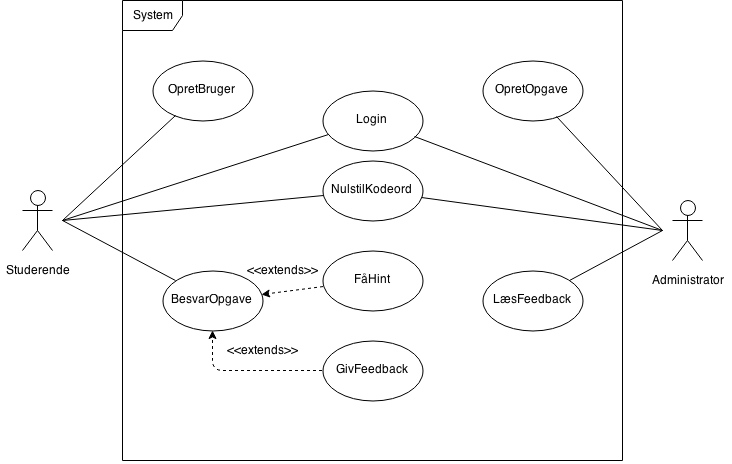
\includegraphics[width=1\linewidth]{figures/UseCaseModel.png}
  \caption{Use case model for vores system.}
  \label{fig:use_case_model}
\end{figure}
\FloatBarrier

\subsection{Use cases}
\label{sub:use_cases}
På Figur \ref{fig:use_case1} ses en beskrivelse af use casen, hvor en studerende opretter sin bruger. Det er en simpel use case, der beskriver i detaljer hvordan processen med at oprette sig som bruger i systemet skal foregå. Inden denne use case er brugeren ikke oprettet i systemet, og når use casen er fuldført har brugeren oprettet sig, er godkendt og er logget ind. Det kombinerer en del af funktionaliteten i én use case. Det kunne godt deles op, men da vi her kun skal beskrive tre overordnede use cases, så har vi valgt at kombineret dem.

\begin{figure}[h]
    \centering
    \begin{tabular}{r p{8cm}}
        \toprule
        \textit{Navn på use-case:} & \verb!OpretBruger! \\
        \hline
        \textit{Deltagende aktører:} & Påbegyndt af en studerende \\
        \hline
        \textit{Hændelser:} & \begin{enumerate}[nolistsep]
            \item En studerende åbner hjemmesiden og klikker på \verb!register!
            \item Den studerende indtaster sine brugeroplysninger, dvs. ku-id og kodeord.
            \item Systemet opretter brugeren, og sender en e-mail med et aktiveringslink.
            \item Den studerende går ind på sin ku-mail klient, åbner mailen og klikker på linket, hvilket aktiverer kontoen.
            \item Den studerende bringes til login-siden.
            \item Den studerende indtaster ku-id og kodeord og klikker \verb!Login!
            \item Der informeres om succesfuldt login, og brugeren bringes til forsiden.
        \end{enumerate}  \\
        \hline
        \textit{Startbetingelse:} & Den studerende har ingen konto, og er ikke logget ind. \\
        \hline
        \textit{Slutbetingelse:} & Den studerende har en aktiveret konto og er logget ind. \\
        \bottomrule
    \end{tabular}
    \caption{Use case omkring oprettelse af bruger.}
    \label{fig:use_case1}
\end{figure}

På Figur \ref{fig:use_case2} ses en beskrivelse af use casen, hvor en studerende svarer på spørgsmål inden for et givet \emph{subject}. Når den studerende har valgt et \emph{subject} vil vedkommende blive stillet en række af spørgsmål tilhørende dette emne. Hver gang den studerende svarer rigtigt på et spørgsmål bliver vedkommende belønnet med point. Dette fortsætter indtil har opnået nok point til at gennemføre det valgte \emph{subject}.

\begin{figure}[h]
    \centering
    \begin{tabular}{r p{8cm}}
        \toprule
        \textit{Navn på use-case:} & \verb!BesvarSpørgsmål! \\
        \hline
        \textit{Deltagende aktører:} & Påbegyndt af en studerende \\
        \hline
        \textit{Hændelser:} & \begin{enumerate}[nolistsep]
            \item Den studerende åbner hjemmesiden.
            \item Vedkommende vælger et \emph{subject} inden for et af de pbne \emph{threshold}.
            \item Systemet præsenterer et spørgsmål for den studerende.
            \item Den studerende angiver sit svar i form af indtastning, afkrydsning eller andet.
            \item Systemet giver respons på svaret, og gemmer alle informationerne i loggen.
            \item Den studerende trykker næste, for at få et spørgsmål mere.
            \item Når den studerende har svaret på nok spørgsmål, har vedkommende gennemført det valgte \emph{subject}, og tages tilbage til forsiden.
        \end{enumerate}  \\
        \hline
        \textit{Startbetingelse:} & Den studerende er logget ind. \\
        \hline
        \textit{Slutbetingelse:} & Den studerende har gennemført et \emph{subject}. \\
        \bottomrule
    \end{tabular}
    \caption{Use case omkring besvarelse af spørgsmål og gennemførelse af subject.}
    \label{fig:use_case2}
\end{figure}

Et af kravene for systemet er, at det skal være enkelt og hurtigt for underviserne i kurset at oprette nye spørgsmål. Da underviserne selv er dataloger, så vil det være optimalt hvis man kan lave spørgsmålene i et struktureret filformat. Vi er blevet enige om at bruge \verb!YAML!\footnote{\url{http://yaml.org}}, derfor er use-casen på Figur \ref{fig:use_case3} meget simpel, og består kun af upload af en YAML fil. Filen der uploades bliver i virkeligheden ikke gemt nogen steder, den bliver bare læst og dataene bliver så brugt til at oprette det nye spørgsmål.

\begin{figure}[h]
    \centering
    \begin{tabular}{r p{8cm}}
        \toprule
        \textit{Navn på use-case:} & \verb!OpretOpgave! \\
        \hline
        \textit{Deltagende aktører:} & Påbegyndt af en administrator \\
        \hline
        \textit{Hændelser:} & \begin{enumerate}[nolistsep]
            \item Administratoren trykker på \verb!Upload File!.
            \item En YAML fil uploades i en formular.
            \item Serveren læser filen og opretter spørgsmålet.
            \item Administratoren informeres om at spørgsmålet er oprettet.
        \end{enumerate}  \\
        \hline
        \textit{Startbetingelse:} & En administrator der er logget ind. \\
        \hline
        \textit{Slutbetingelse:} & Det nye spørgsmålet er oprettet. \\
        \bottomrule
    \end{tabular}
    \caption{Use case omkring oprettelse af opgaver.}
    \label{fig:use_case3}
\end{figure}
\FloatBarrier

\subsection{Klassediagram}
På Figur \ref{fig:class_diagram} kan man se vores klassediagram. Størstedelen af klasserne har at gøre med opgaverne og deres inddeling i forskellige grupper samt de forskellige typer af opgaver der findes. Derudover er der et par klasser der har at gøre med den log der føres over de studerendes opgavebesvarelser, for at de kursusansvarlige kan følge med i hvad der går godt og mindre godt. Endeligt er der en klasse for brugere af systemet.

\begin{figure}[h]
    \centering
    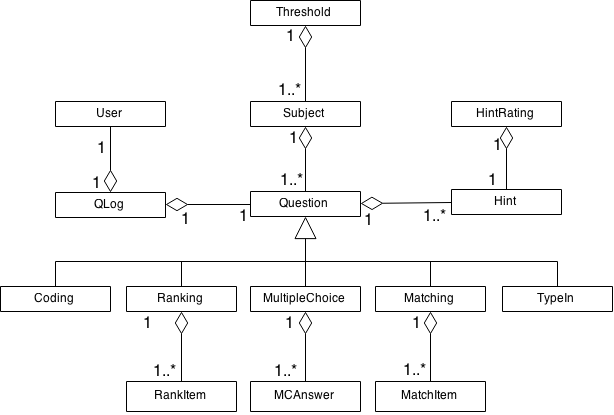
\includegraphics[width=1\linewidth]{figures/ClassDiagram.png}
    \caption{Klassediagram af problemområdet}
    \label{fig:class_diagram}
\end{figure}
\FloatBarrier

\subsection{BCE-model}
På Figur \ref{fig:bce_model} kan man se vores BCE model. Modellen har to entity-objekter, fire controller-objekter samt tre boundary-objekter.

\begin{figure}[h]
  \centering
  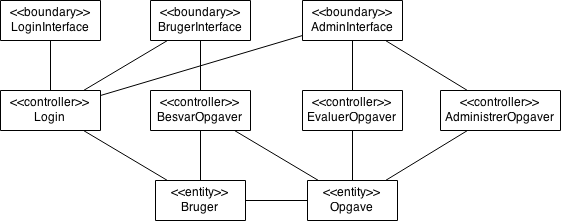
\includegraphics[width=1\linewidth]{figures/BCE-Model.png}
  \caption{BCE model for vores system.}
  \label{fig:bce_model}
\end{figure}

De to entity-objekter er \emph{Bruger} og \emph{Opgave}. \emph{Bruger} indeholder informationer om hver enkelt bruger, så som login-oplysninger, hvor vidt brugeren er studerende eller admin samt hvilke \emph{subjects} brugeren allerede har gennemført. \emph{Opgave} indeholder alle informationerne om \emph{thresholds}, \emph{subjects} og opgaver, samt statistik omkring hvordan det er gået når de studerende har løst opgaverne.

Modellen har tre boundary-objekter, hvor det første man vil møde når man indlæser siden er \textit{login}-brugergrænsefladen, der sammen med \emph{login}-controlleren sørger for at logge brugerne ind i systemet. Derefter vil man så enten have adgang til \emph{Bruger}-grænsefladen eller \emph{Admin}-grænsefladen afhængig af hvad ens status er, og derfra har man adgang til en række controllers.

Modellen har fire controller-objekter, hvor den første er \emph{login}-controlleren der som tidligere nævnt står for at logge brugere ind i systemet. Som studerende vil man have adgang til \emph{BesvarOpgave}-controlleren, der snakker sammen med \emph{Bruger} og \emph{Opgave} og sørger for at stille brugeren de rigtige opgaver. Som admin vil man have adgang til to controllers, nemlig \emph{EvaluerOpgave}-controlleren og \emph{AdministrerOpgave}-controlleren. \emph{EvaluerOpgave}-controlleren snakker sammen med \emph{Opgave} og giver en adgang til de forskellige slags statistik der bliver samlet om opgaverne, og \emph{AdministrerOpgave}-controlleren snakker ligeledes sammen med \emph{Opgave} og giver en adgang til at slette eller ændre i eksisterende opgaver samt tilføje nye.
\FloatBarrier

\subsection{Sekvens-diagrammer}
I dette afnit er der lavet sekvensdiagrammer over de tre use cases der er beskrevet i Afsnit \ref{sub:use_cases}. De funktionskald der fremgår af sekvensdiagrammerne er ikke nødvendigvis reelle funktioner i vores applikation, men er nærmere brugt for at beskrive hvad der sker.
På Figur \ref{fig:opret_bruger_sekvens} kan man se sekvens-diagrammet for den første use case, der beskriver hvordan en studerende opretter sig som bruger i systemet. Her indgår to adskilte sessioner. I den første opretter brugeren sig i systemet, og systemet sender så en email til brugeren. I næste session klikker brugeren på et link i denne email, og brugeren bliver så aktiveret i systemet. Derefter logger brugeren ind, får at vide at det er lykkedes, og use casen er så færdig.

\begin{figure}[h]
    \centering
    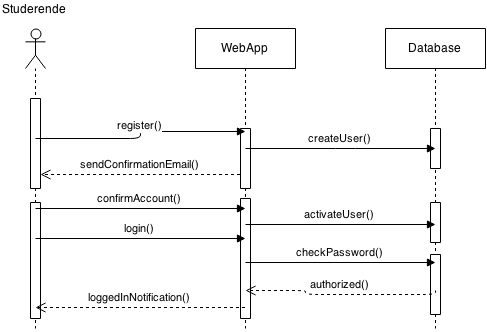
\includegraphics[width=1\linewidth]{figures/OpretBrugerUseCase.png}
    \caption{Sekvensdiagram over opretning af bruger}
    \label{fig:opret_bruger_sekvens}
\end{figure}

På Figur \ref{fig:svar_sekvens} kan man se sekvens-diagrammet for den anden use case, der beskriver hvordan en studerende vælger et \emph{subject} og dernæst besvarer spørgsmål indtil det valgte \emph{subject} er gennemført. Løkken viser at der kan komme flere end ét spørgsmål efter det første.

\begin{figure}[h]
    \centering
    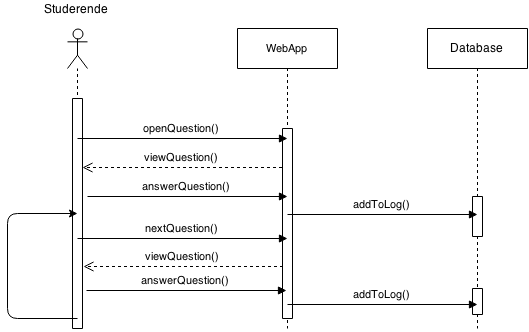
\includegraphics[width=1\linewidth]{figures/SvarUseCase.png}
    \caption{Sekvensdiagram over besvarelse af spørgsmål og gennemførelse af subject.}
    \label{fig:svar_sekvens}
\end{figure}

På Figur \ref{fig:opret_sp_sekvens} kan man se sekvens-diagrammet for den tredje use case, der beskriver hvordan en administrator opretter et nyt spørgsmål i systemet. Dette sekvensdiagram er stort set linært, da der ikke sker mere end at der uploades fil, filen læses og spørgsmålet tilføjes, og der gives respons om hvorvidt at spørgsmålet er oprettet korrekt.

\begin{figure}[h]
    \centering
    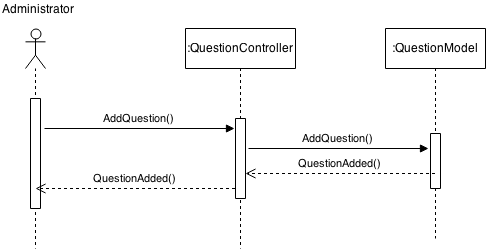
\includegraphics[width=1\linewidth]{figures/OpretSporgsmalUseCase.png}
    \caption{Sekvensdiagram over opretning af spørgsmål}
    \label{fig:opret_sp_sekvens}
\end{figure}
\FloatBarrier

\section{Systemdesign}
\label{sec:systemdesign}
I dette afsnit beskrives de forskellige apsekter af vores systemdesign. Til sidst i afsnittet gennemgås de dele vi ikke har nået at gennemføre/implementere.

\subsection{Valg af frameworks}
\label{sub:valg_af_frameworks}
Som før omtalt i Afsnit \ref{sec:formal_og_rammer} har vi valgt at bruge frameworket \emph{Flask} som grundlag for vores webapplikation, der på deres egen hjemmeside\footnote{\url{http://flask.pocoo.org/}} er beskrevet som et såkaldt \emph{microframework}. Det betyder at der ikke følger mange af de ting med som der gør i mange større webframeworks. Flask tilbyder kun HTTP routing og templating\footnote{Templating er en måde at vise data fra et programmeringsprog inde i et dokument.}. Resten skal man selv finde andre biblioteker til. Vi har valgt det, da der så ikke er så meget, at skulle sætte sig ind i, og det giver mere frihed til at udforme applikationen som kunden og vi synes er bedst.

\subsection{Strukturering}
\label{sub:strukturering}
I nogle udviklingsmiljøer er der typisk givet en struktur af kodebasen på forhånd. Det gælder f.eks. mange gange når man bruger store frameworks som Django til Python eller Play til Java. Der er nogle konventioner for hvilke klasser der skal i hvilke mapper, og til hvordan konfigurationsfiler skal struktureres. Det er med til at sikre en god strukturing af koden. Frameworket Flask, som vi har valgt at bruge, har ikke sådanne konventioner. Alt kode kunne i teorien placeres i én stor fil hvis man ville. Derfor har vi været omhyggelige med at organisere moduler og klasser i forskellige filer og mapper på en sådan måde at det er overskueligt og forståeligt.

Det giver god mening som den første nedbrydning at dele applikationen op i moduler, som hver især indkapsler adskildt funktionalitet. Det beskrives også i kapitel 6.3 i \cite{OOSE} hvordan man får delt et system op, så kohæsionen mellem moduler bliver så lille som mulig. Ud fra kravspecifikationen har vi nedbrudt det i fire moduler; \texttt{user, admin, question} og \texttt{log}.

\texttt{User} modulet håndterer den del der har at gøre med brugerlogins, og alt der hører med af oprettelse, ændring og nulstilning af kodeord osv. \texttt{Admin} modulet håndterer den del der har at gøre med administration af spørgsmål, \emph{subects}, \emph{thresholds} og brugere. \texttt{Log} modulet håndterer den del der har at gøre med logning af statistik fra spørgsmålbesvarelser, samt visning af denne. Endelig håndterer \texttt{question} modulet den del der har at gøre med spørgsmål, \emph{subjects} og \emph{thresholds}, både selve opbygningen af hele spørgsmål-strukturen samt visning og besvarelse af spørgsmål.

Denne opdeling har gjort at vi nemmere har kunnet takle problemer uafhængigt af hinanden, og derved har kunnet udvikle mere effektivt.

\subsection{Databasedesign}
\label{sub:databasedesign}
På Figur \ref{fig:er_diagram_question} er ER-diagrammet for hele spørgsmål-aspektet af vores database. Det er minder en del om klassediagrammet over vores problemområde som ses på Figur \ref{fig:class_diagram}, dog er det her mere konkret vist hvilke atributter de enkelt klasser har. På diagrammet ses strukturen for hvordan spørgsmålene er inddelt. Man kan se hvordan et \emph{Question} hører til et \emph{Subject}, der igen hører til et \emph{Threshold} og så videre. Vi prøver også at vise den modulære struktur hvor vi har ladet nye typer spørgsmål nedarve fra den generaliserede type.

\begin{figure}[h]
    \centering
    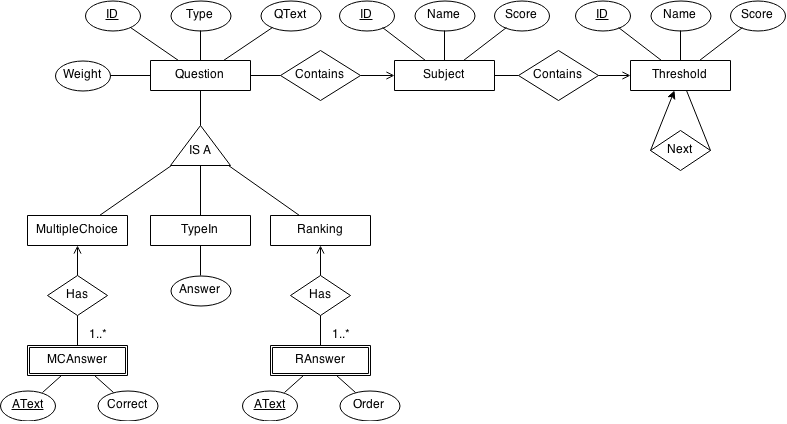
\includegraphics[width=1\linewidth]{figures/er_diagram/Qdb.png}
    \caption{ER-diagram over delen af databasen hvor spørgsmålene hører til.}
    \label{fig:er_diagram_question}
\end{figure}

Log-aspektet af vores database er rimelig simpel, idet at vi blot har to tabeller; \emph{QLog} og \emph{HintRatings}. Hver gang en studerende vælger et emne og begynder at svare på spørgsmål bliver der gemt en masse informationer om det i QLog-tabellen. I den anden tabel bliver det gemt når en studerende giver en vurdering af et specifikt hint.

Det tredje aspektet af vores database er brugere. Vi har en \emph{Users} tabel, hvor alt informationen om brugerne og deres kontoer bliver gemt, deriblandt også hvilken rolle de har i systemet.
\FloatBarrier

\subsection{Brugere}
\label{sub:brugere}
Modulet \texttt{user} håndterer brugere. Vi har implementeret funktionalitet som vi synes børe være i et brugerhåndteringssystem. Der er følgende features:

\begin{itemize}
    \item Log ind og log ud
    \item Oprettelse af brugere med email-godkendelse via. KU-mail
    \item Skift af password
    \item Nulstilling af password
\end{itemize}

For at det ikke skal være muligt at se brugeres password, gemmer vi en hashet udgave af det i databasen vha. password hashing funktionaliteten der følger med \verb!Flask!. Den benytter hashing algoritmen \verb!SHA1! som er implementeret i pythons standardbibliotek. Dette er vigtigt for os, da det er vigtigt at hashing algoritmen er til at stole på.

Vi godkender brugere ved at sende en email til deres KU-mail. I denne mail er der en token som kan afkodes til brugerens KU-id, så det er kun præcis den token der fungerer. Vi bruger samme teknik til nulstilning af passwords, for at være sikker på at det er den korrekte bruger der får lov at nulstille passwordet eller godkende brugeren.

Ændring af password er trivielt, man skal bare være sikker på at brugeren er logget ind først.

Vi implementerer forskellige brugertyper med flag i databasen. For at gøre det nemt at lave adgangskontrol på views, har vi implementeret en decorator som pakker hvert view ind. Det ser ud på følgende måde:

\begin{python}
@app.route('/admin')
@role_must_be('admin')
def admin_index():
    return render_template('admin/index.html')
\end{python}

for et view der f.eks. kunne vise admin siden. Den tjekker så om den nuværende bruger der er logget ind har rollen \verb!admin!.

\subsection{Spørgsmål}
\label{sub:sporgsmal}
Ud fra ER diagrammernes nedarvningshieraki, har vi implementeret dem som Python klasser der alle nedarver fra en generel klasse \verb!Question!. I underklasserne er der så alle de attributter der adskiller spørgsmåltyperne fra hinanden. I et kodespørgsmål er der for eksempel tilføjet attributterne \verb!code! og \verb!exec_name!. Den første er kodestumpen der skal modificeres, og det andet er den eksekverbare fil der findes på serveren til at vurdere brugerens svar på opgaven. For ikke at skulle ændre i logikken til at vise spørgsmål, bruges en polymorf metode \verb!render_question!. Den sørger for at generere HTML'en for et givet spørgsmål, samt tjekke om svaret brugeren indsender er korrekt. Tricket er så, at når man laver en ny underklasse af \verb!Question!, så skal man kun skrive én ny metode til at generere et view og tjekke svaret. Det er et led i, at vi gerne vil gøre koden så modulær som muligt.

Et af kravene i kravspecifikationen var, at man kunne oprette spørgsmål fra et semistruktureret filformat som f.eks. \verb!YAML!. Til dette har vi brugt et \emph{Factory Method Pattern}. Det er en simpel version af det \emph{Factory Pattern} der beskrives i kapitel 8 i Bruegge og Dutoit\cite{OOSE}. Vi har implementeret en statisk metode, som sørger for at lave det rigtige \verb!Question! ud fra et givet python \verb!dict!. Vi slipper derved for at tænke alt for meget på underklasser fordi man i python har \emph{duck-typing}, hvilket vil sige, at interfaces er implicitte. Det gør at man kan returnere det specifikke objekt i stedet. Den implementerede funktion hedder \verb!from_dict!, og returnerer det spørgsmål der er blevet oprettet ud fra det givne data. Vi kan på den måde bruge mange forskellige strukturerede filformater, da mange biblioteker tager en fil ind, og outputter en \verb!dict!.

Da \emph{thresholds} har en naturlig rækkefølge, så er de lidt mere komplicerede. Man kan ikke bare indsætte dem ind i databasen, da SQL ikke garanterer nogen rækkefølge. Det har givet os to muligheder for at implementere det. Man kan enten give hvert threshold et tal for hvilket nummer i rækkefølgen af \emph{thresholds} det enkelte \emph{threshold} er. En anden mulighed, som er den vi har valgt, er, at hvert \emph{threshold} har en pointer til det næste \emph{threshold} object i rækken. Det gør det meget simpelt at vedligeholde databasen, og indsætte data. I praksis betyder det, at hvert \emph{threshold} har en \verb!next! attribut, og for finde de næste thresholds, så følger man bare deres pointers.

Et andet krav er, at man skal kunne få hints til opgaverne. For at man ikke kan snyde, og se hints inden man har bedt om dem, så sender vi dem dynamisk til brugeren. Det vil sige at de injiceres på hjemmesiden mens vedkommende er i gang med at løse opgaven. Vi kan så på serversiden holde øje med hvor mange hints den pågældende bruger har bedt om, og gemme det i loggen. Det foregår med teknologien \verb!AJAX!, som går ud på, at man sender et asynkront HTTP-request til serveren, som så sender data tilbage. Hjemmesiden ændres så dynamisk, sådan at dataene sættes ind på siden uden at den genindlæses.

Et af de mere komplicerede krav til systemer er, at det skal være forbedredt til kodespørgsmål, som skal tjekkes med et program på severen. Dette er noget som vores kunder selv vil implementere, så vi har specificeret en grænseflade mellem vores applikation og systemet, som betyder at systemet kører et script der hører til et spørgsmål, og der fødes så information frem og tilbage. Dette skal også være behageligt for brugeren, så ved kodespørgsmål vises et redigeringsvindue der fremhæver \verb!F#! syntaks. Til dette bruges JavaScript editoren CodeMirror\footnote{\url{https://codemirror.net/}}.

\subsection{Admin}
\label{sub:admin}
Vores admin modul er mere eller mindre direkte importeret fra flask modulet \emph{admin}, og udover at tilføje funktionalitet til uploading og læsning af yaml-filer har vi ikke gjort meget mere med det. Den primære funktion af modulet er at det gør det muligt at oprette et view for hver tabel i databasen, hvor man så kan se hvilket rækker og kolonner der optræder i tabellen, samt oprette, ændre og slette i dataene. Vi har dog opbygget vores database ved hjælp af SQLAlchemy, hvilket vi har fundet ud af ikke arbejder så godt sammen med admin modulet, så meget af funktionaliten fungerer ikke rigtigt.

Vi har dog som nævnt også tilføjet funktionalitet til at uploade og indlæse filer. Det fungerer på den måde, at når en admin uploader en fil, så bliver den læst af serveren, hvis det da er en korrekt udfyldt yaml fil. Informationerne i filen bliver så brugt til at oprette et nyt spørgsmål, \emph{subject} eller \emph{threshold}, som så tilføjes til databasen. Som det ser ud lige nu, bliver filen ikke gemt nogen steder, når den er blevet læst.

Lige fra da vi implementerede admin modulet, har det dog også kun været en midlertidig løsning, som vi gerne ville have arbejdet videre på. Vi har dog aldrig rigtig haft tiden til det. Kunden ville gerne have haft et admin system med mere fokus og funktionalitet baseret på yaml filerne, og hvor det skulle være nemt at se hvad det lavede og ændrede. Det har vi også haft nogle tanker omkring hvordan vi ville gribe an. Vi er dog ikke nået videre med det.

\subsection{Log}
\label{sub:log}
Loggen for vores system er på nuværende tidspunkt meget simpelt implementeret. Det fungerer simpelthen på den måde, at hver gang en studerende besvarer et spørgsmål, så bliver der gemt en masse informationer i loggen. Det er for eksempel hvilken bruger og hvilket spørgsmål der er tale om, et tidsstempel, hvad brugeren har svaret, hvor mange hints brugeren brugte og så videre. Alt denne information bliver så gemt i en stor tabel i databasen. Inde på hjemmesiden er der så et link der hedder \emph{log}, som tager en til en side hvor man kan se disse informationer.

Vores implementation af en log er ret simpel, og på længere sigt ville man naturligvis gerne have en mere omfattende lagring af informationer, og især nogle mere brugbare og informative måder at se dataene i loggen på, for eksempel i form af diverse statistikker og grafer. Det er dog igen noget vi ikke har nået at komme så meget videre med på den tid vi har haft.

\subsection{Udestående design- og implementationsopgaver}
\label{sub:udestaende_design_og_implementationsopgaver}
De ting vi mangler at implementere er kunne lave mere komplicerede statistiske operationer på de loggede data. Dette kunne for eksempel væreat finde de spørgsmål de studerende har svært ved, eller at finde spørgsmål der ikke er optimale. Vi mangler også at admin interfacet bliver forbedret, så det bliver mere brugervenligt. Vi mangler også at få kodespørgsmålene implementeret korrekt, men der mangler vi også noget arbejde fra vores kunder.

Et krav, der er kommet frem senere, men som vi ikke har haft tid til at kigge på er, at systemet skal kunne håndtere flere kurser på flere årgange. Det er en større designopgave, og derfor ikke noget vi har tid til i denne omgang.

\section{Program- og systemtest}
\label{sec:program_og_systemtest}
I dette afsnit uddybes vores teststrategi, og det beskrives hvordan testene er forløbet.

\subsection{Unittests}
\label{sub:unittests}
For at det skal være så nemt og smertefrit som muligt at teste, så bruger vi et automatisk unittest værktøj. Ifølge \cite{COCO}, så er automatiske tests den eneste reelle måde at teste på. En af fordelene i vores tilfælde er, at hvis man laver mange ændringer i koden, som der ofte er, når man arbejder agilt, så er det vigtigt at man kan køre testene hurtigt og nemt efter hver ændring af koden. Vi bruger det inkluderede testbibliotek i \verb!Python! nemlig \verb!unittest!\footnote{\url{https://docs.python.org/2/library/unittest.html}}. Det virker på samme måde som \verb!JUnit! i \verb!Java!, hvor man skriver testmetoder i en testklasse.

For at være sikker på at vores tests er dækkende, så bruges et værktøj der måler dækningsgraden (Afsnit 11.4.3 i \cite{OOSE}) af vores tests. Det giver et mål for hvor gode testene er. Dette værktøj er \verb!coverage!\footnote{\url{http://nedbatchelder.com/code/coverage/}}. Det kan også generere rapporter, der giver et overblik over koden, og visuelt viser hvilke dele af koden vores tests dækker, og hvilke der delvist eller slet ikke er dækket.

På Figur \ref{fig:testcoverage} ses en udskrift af testrapporten. Her kan man see hvilke moduler af koden, som er dækket tilstrækkeligt af tests, og hvilke der måske stadig har nogle mangler.

\begin{figure}[h]
    \centering
    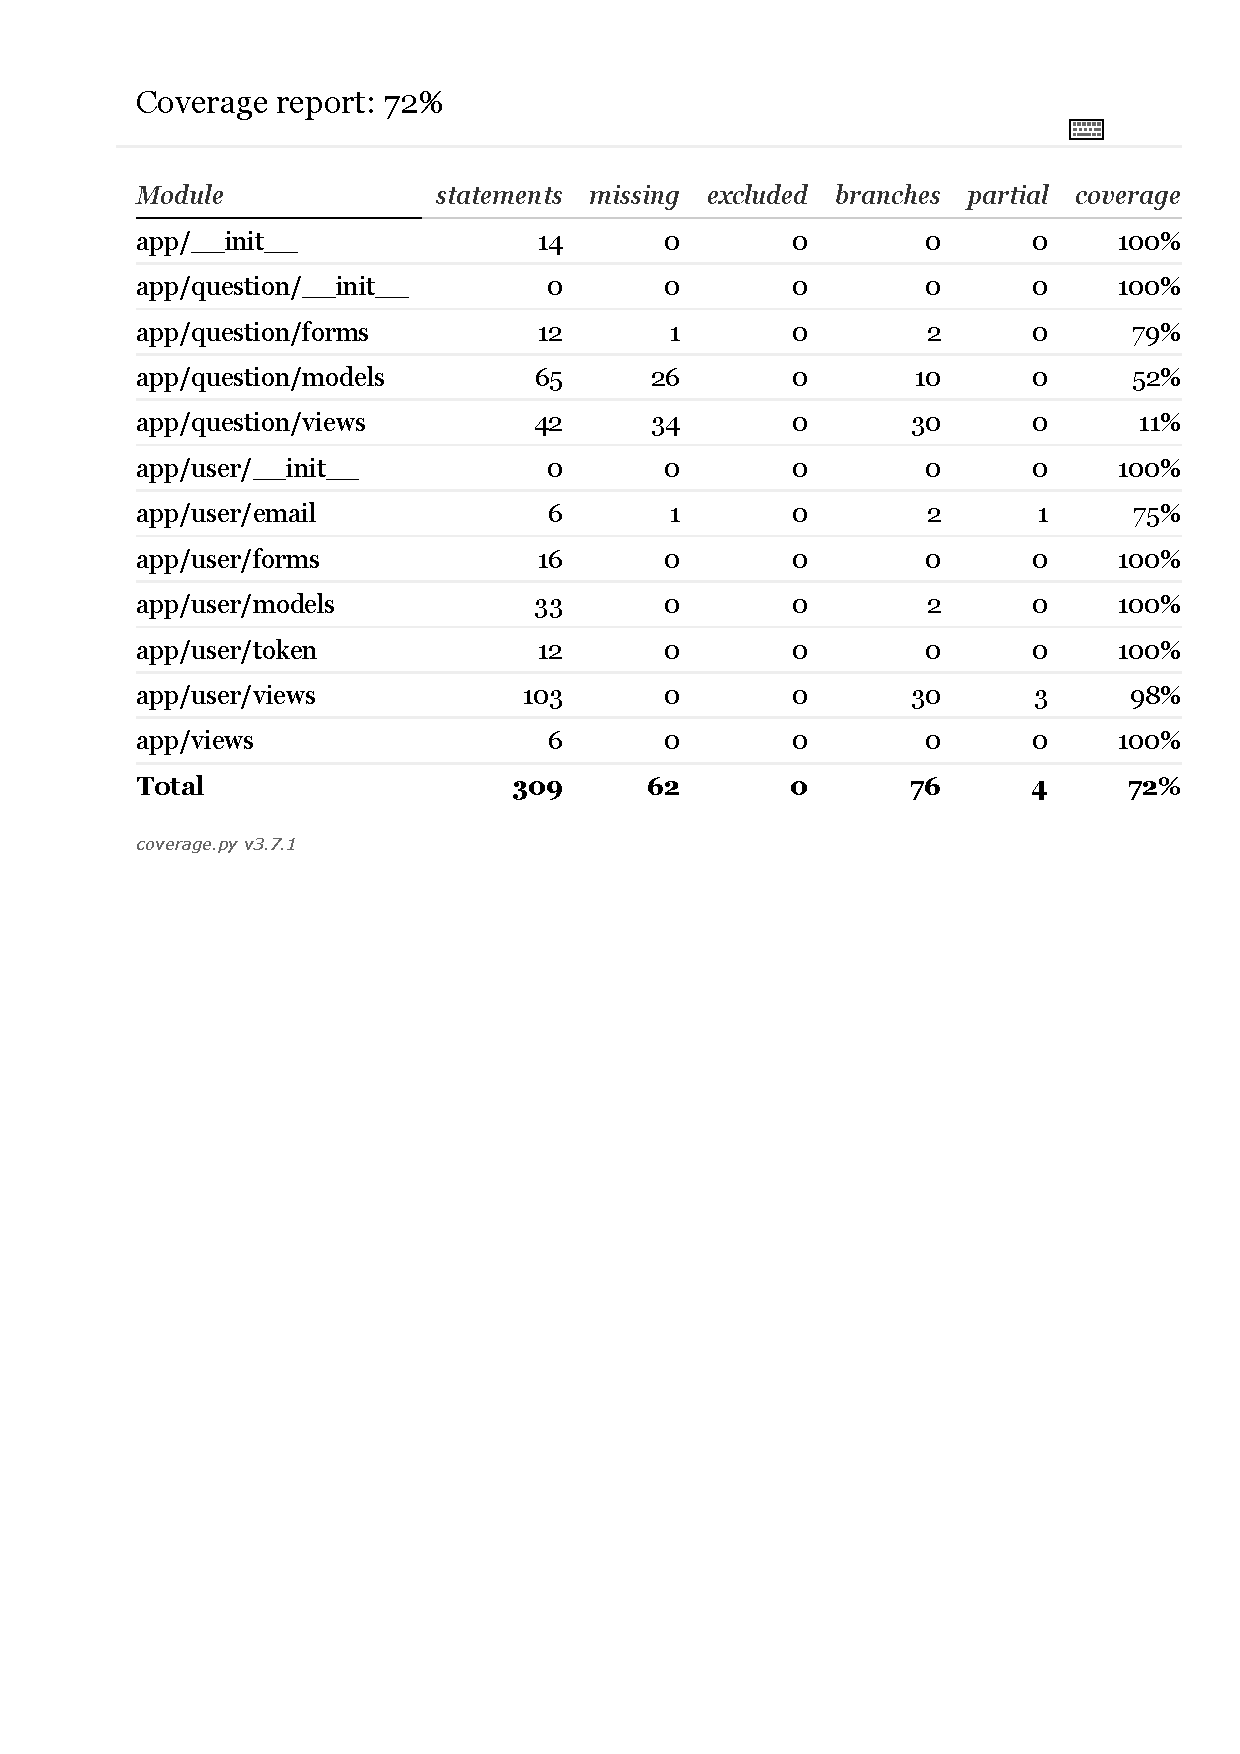
\includegraphics[width=1\linewidth]{figures/testcoverage.pdf}
    \caption{Oversigt over dækningsgraden af unittests. Det ses også hvor mange udtryk der er dækket af tests.}
    \label{fig:testcoverage}
\end{figure}

På Figur \ref{fig:code_coverage} ses hvordan værktøjet viser hvilke dele af koden der er dækket af tests, og hvilke der ikke er.

\begin{figure}[h]
    \centering
    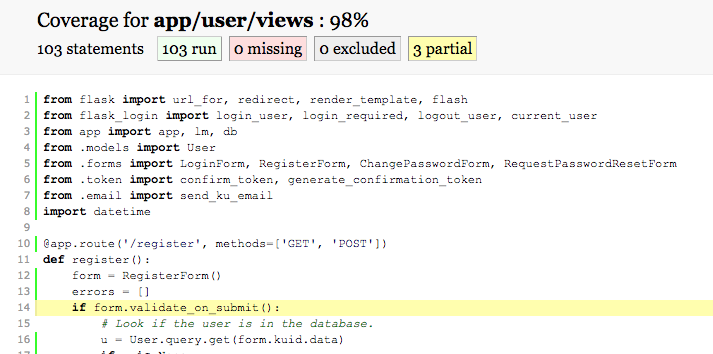
\includegraphics[width=1\linewidth]{figures/code_coverage.png}
    \caption{Eksempel på en grafik fremstilling, hvor et udtryk der kun delvist er dækket af tests fremhæves med gult.}
    \label{fig:code_coverage}
\end{figure}

\FloatBarrier

\subsection{Integrationstests}
\label{sub:integrationstests}
Vores integrationstests foregår med samme værktøjer som vores unittests. Forskellen ligger i, hvordan testene er designet. I integrationstests testes at sammenspillet med modulerne er som ønsket, og at man kan bruge flere funktionaliteter på en gang. Vi har ikke haft tid til at skrive mange tests, men vi har tests der opretter databaseelementer, logger en bruger ind og åbner spørgsmål. Undervejs tjekkes så at alt er i overensstemmelse med kravspecifikationen, og at der vises præcist hvad der skal på hjemmesiden. Her er det ikke så vigtigt med dækningsgraden af koden, men det er vigtigt at punkter fra kravspecifikationen testes. Det kan for eksempel være, at brugeren skal kunne logge ind og starte med at besvare spørgsmål.

\subsection{Usability-tests}
\label{sub:usability_tests}
Vi har ladet den ene af vores kunder, Martin, afprøve vores system, og noteret hans kommentarer ned.

Det første der blev kommenteret på var selve layoutet og navigationen af vores webside. Når man gik ind på diverse sider var det ikke nemt at komme tilbage igen hvis man ønskede det, uden direkte at skulle benytte browserens funktion til at gå tilbage. Det var heller ikke åbenlyst at \emph{PoP} logoet i øverste venstre hjørne tog en tilbage til forsiden, eller hvad \emph{Overview} linket inde på admin siden betød.

Det er en pointe som vi helt klart vil tage til os, og vi er også enige i at navigationen af hjemmesiden ikke er helt optimal. Som udviklere ved vi naturligvis hvad enhver knap og funktion gør, men det er naturligvis ikke tilfældet for brugere, og det skal vi selvfølgelig huske at tage hensyn til.

Derudover drejede det sig i høj grad os om selve admin interfacet. Halvdelen af funktionaliteten i vores admin modul virker ikke rigtig sammen med vores database, og den anden halvdel er ikke altid helt åbenlys at få til at virke. Martin så hellere at alt håndtering af spørgsmål og lignende foregik ved at man tilføjer og ændrer i YAML filer, frem for at man skal bruge et webinterface.

Det er igen en kritik vi er meget enige i, admin-interfacet har lige fra det blev indført stået højt på listen over ting vi godt ville have ændret, vi har bare ikke lige haft tiden til det, da vi i stedet har prioriteret at lave de ting der helt manglede at blive lavet.

\section{Brugergrænseflade og interaktionsdesign}
\label{sec:userinterface}

I dette afsnit beskrives vores brugergrænseflade og hvordan der interageres med den. Derudover vises der skærmbilleder af den centrale funktionalitet og diagrammer der viser flowet gennem applikationen.

\subsection{Screenshots}
\label{sub:screenshots}
I dette afsnit ses screenshots af brugergrænsefladen for de vigtigste dele af vores projekt. De optræder i en rækkefølge der illustrerer dynamikken i en studerendes interaktion med vores system. Først kommer der et afsnit om login, dernæst om de studerendes del, og til sidst om admin delen af vores projekt.

\subsubsection{Login}
\label{subsub:screenshots_login}
På Figur \ref{fig:screenshot_login} ses et screenshot af den første del af vores brugergrænseflade en studerende vil møde, nemlig en login skærm. Hvis man allerede er registreret som bruger kan man her indtaste sit KU-id og sit valgte kodeord, og dermed logge på systemet. Hvis man ikke er oprettet som bruger er der et link der tager en videre til registrering.

\begin{figure}[htpb]
    \centering
    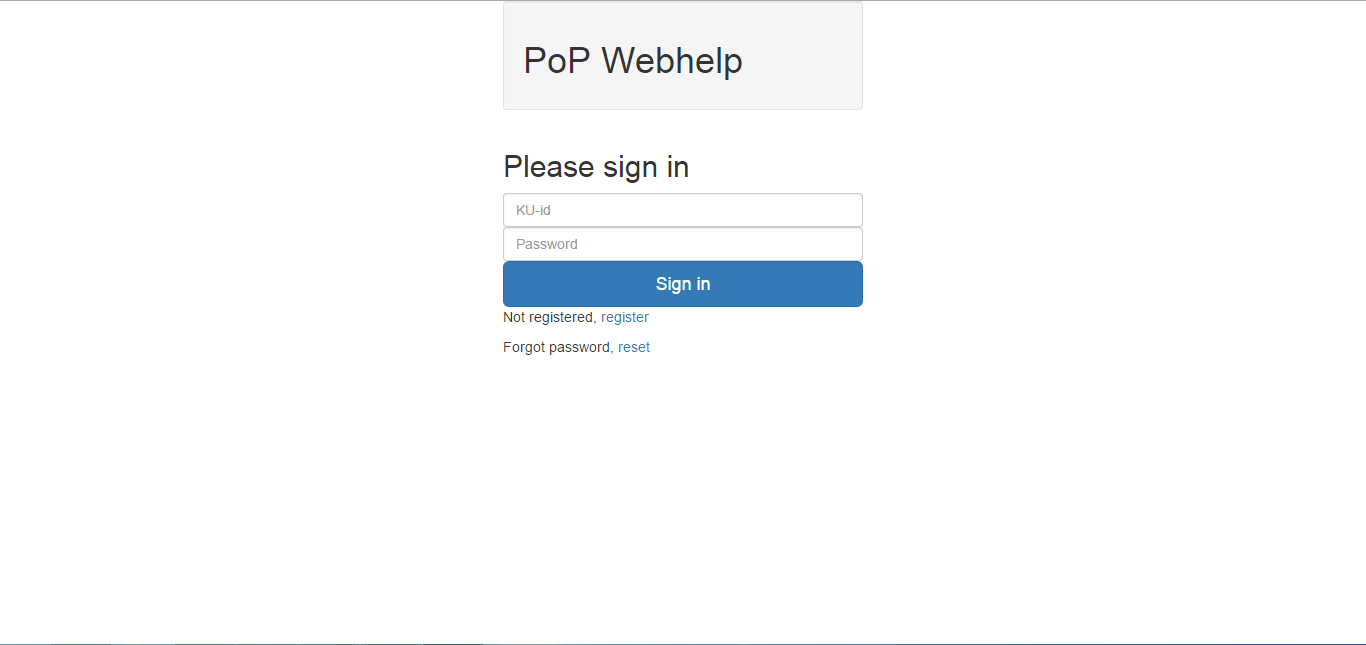
\includegraphics[width=1\linewidth]{figures/interface/login.png}
    \caption{Screenshot af login-siden.}
    \label{fig:screenshot_login}
\end{figure}

På Figur \ref{fig:screenshot_register} ses registreringssiden. Her kan man indtaste sit KU-id, vælge sig et kodeord og registrere sig. Systemet sender så en mail til den relevante KU-mail med et verificeringslink, og så snart den studerende har trykket på linket er vedkommende klar til at logge på systemet.

\begin{figure}[htpb]
    \centering
    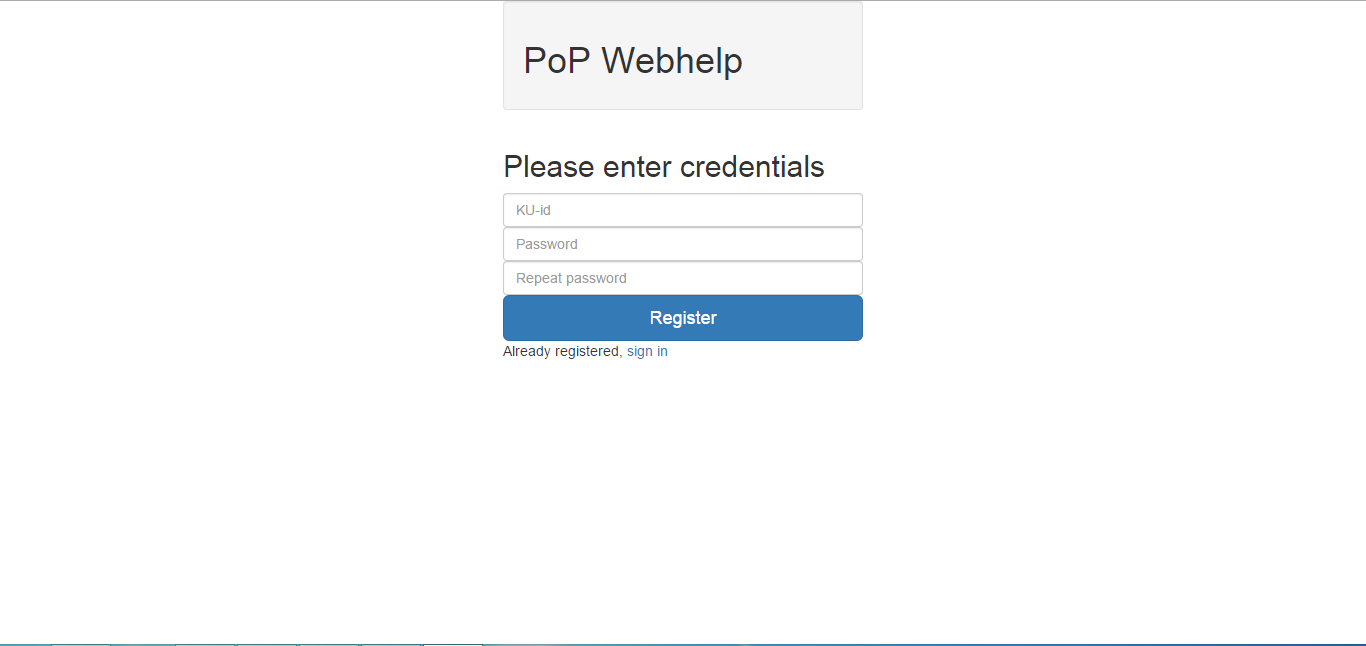
\includegraphics[width=1\linewidth]{figures/interface/register.png}
    \caption{Screenshot af registrerings-siden.}
    \label{fig:screenshot_register}
\end{figure}

\FloatBarrier

\subsubsection{Studerende}
\label{subsub:screenshots_student}
Når en studerende har logget sig ind i systemet vil vedkommende blive taget til index siden, som kan ses på Figur \ref{fig:screenshot_overview}.  I toppen siden ses en navigationsbar, hvor man bl.a. kan se hvem man er logget ind som, man kan logge ud og man kan ændre sit password. Der er desuden i venstre side et slags logo hvor man kan trykke for at blive taget tilbage til forsiden.

På forsiden kan den studerende få et overblik over de forskellige \emph{thresholds} og de dertil hørende \emph{subjects}. De \emph{thresholds} som den studerende har låst op for er grønne, og ved at trykke på de \emph{subjects} der hører til disse kan den studerende begynde at svare på spørgsmål. De \emph{thresholds} som den studerende ikke har låst op for er røde, og de detilhørende \emph{subjects} kan ikke trykkes på.

\begin{figure}[htpb]
    \centering
    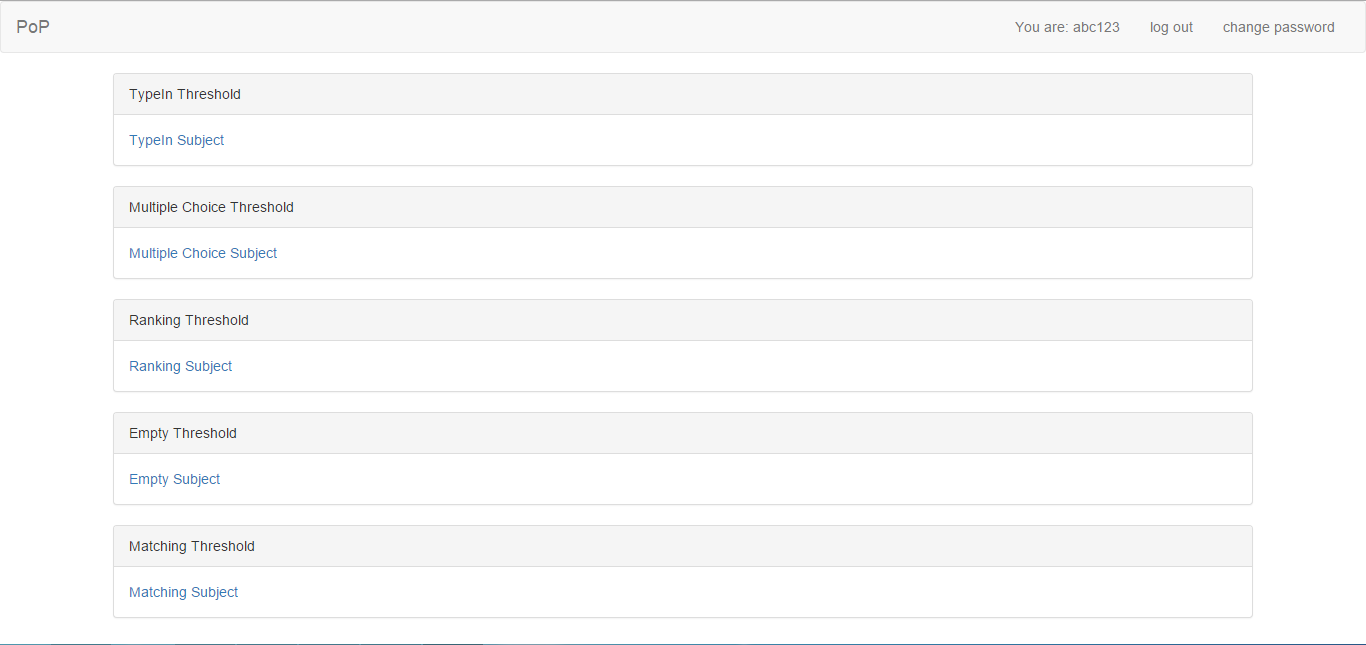
\includegraphics[width=1\linewidth]{figures/interface/overview.png}
    \caption{Screenshot af index-siden.}
    \label{fig:screenshot_overview}
\end{figure}

På Figur \ref{fig:screenshot_subject} ses \emph{subject} siden, hvor den studerende kan læse om det valgte \emph{subject}, og hvis det virker interessant, trykke på knappen og begynde at løse opgaver inden for dette \emph{subject}.

\begin{figure}[htpb]
    \centering
    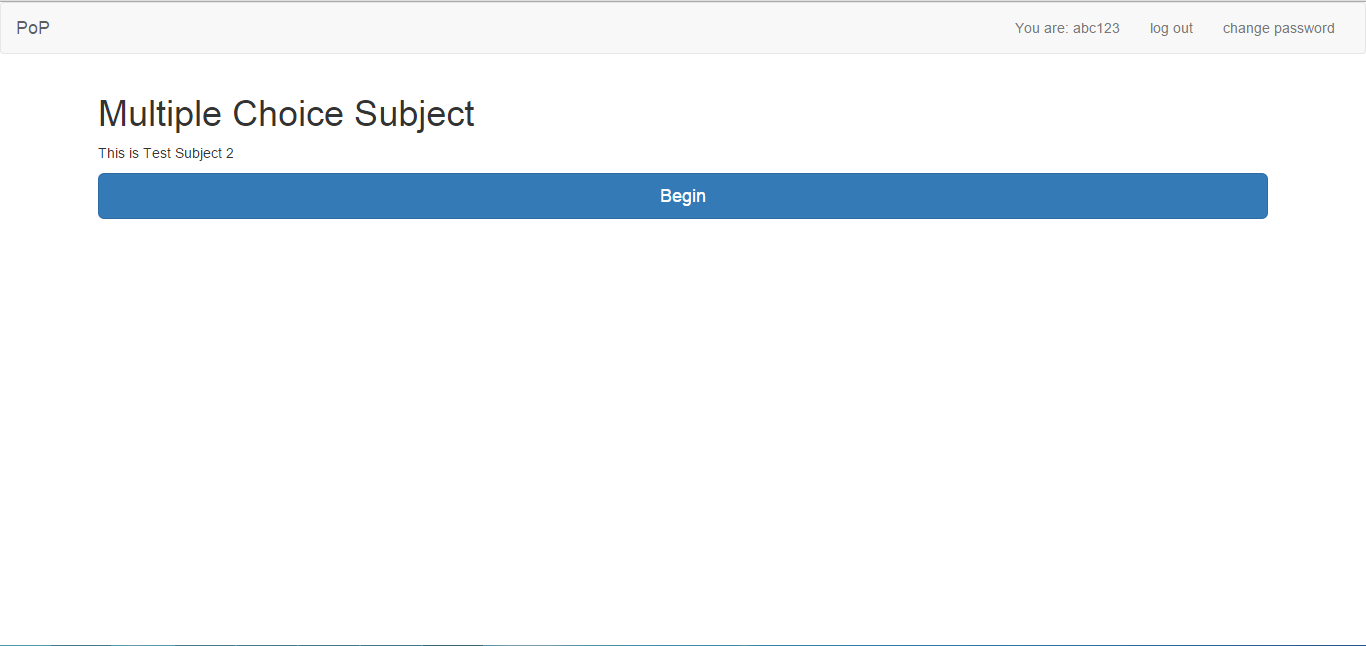
\includegraphics[width=1\linewidth]{figures/interface/subject.png}
    \caption{Screenshot af \emph{subject}-siden.}
    \label{fig:screenshot_subject}
\end{figure}

Når den studerende har trykket \emph{begin} vil vedkommende blive stillet en række opgaver, f.eks. multiple choice opgaver som den der kan ses på Figur \ref{fig:screenshot_question}. Den studerende kan så afgive sit svar, enten ved at indtaste et svar, afkryde de korrekte bokse eller trække svarmulighederne hen på de korrekte positioner, og trykke på \emph{answer} knappen. Der er desuden mulighed for at den studerende kan få hints til opgaven, hvis det skulle være nødvendigt, ved at trykke på \emph{Get hint} knappen.

\begin{figure}[htpb]
    \centering
    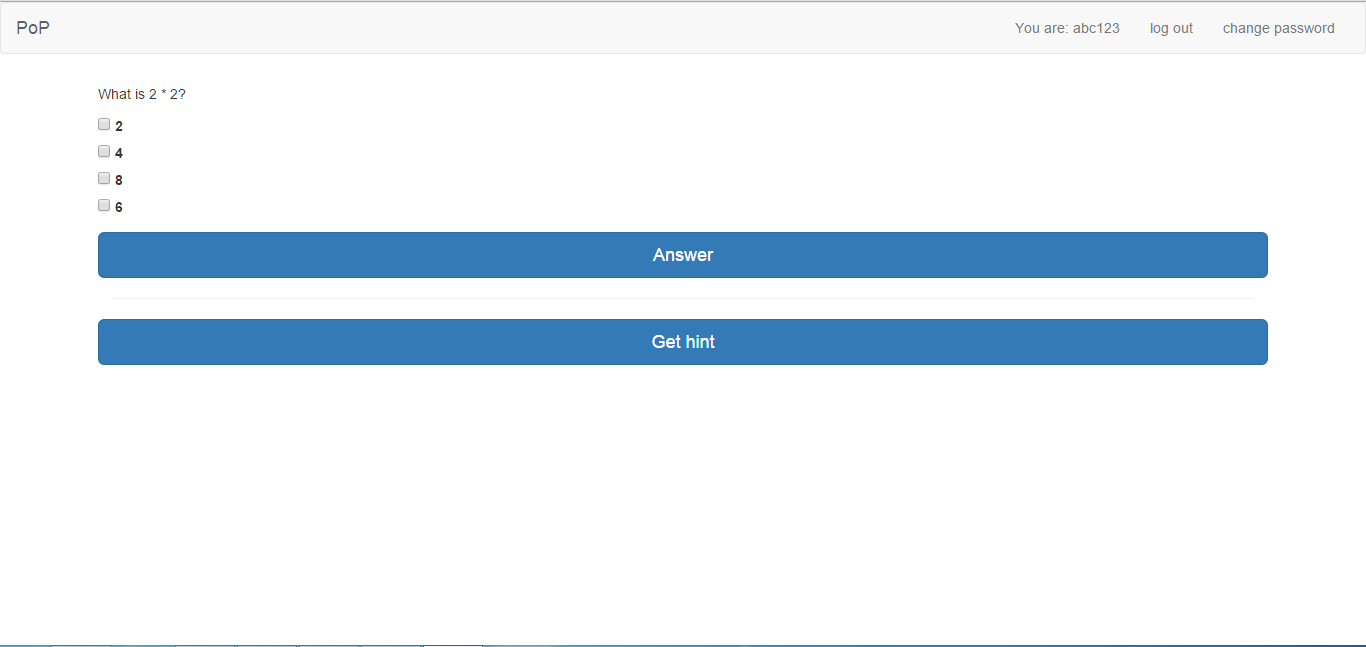
\includegraphics[width=1\linewidth]{figures/interface/question.png}
    \caption{Screenshot af spørgsmåls-siden.}
    \label{fig:screenshot_question}
\end{figure}

Når den studerende har svaret på et spørgsmål vil vedkommende blive taget til svar-siden, som kan ses på Figur \ref{fig:screenshot_answer}. Her får den studerende feedback på sit svar, der kan variere fra en helt simpel besked i form af rigtigt eller forkert til et mere detaljeret svar der f.eks. kunne indeholde en relevant stack trace hvis den studerende har skrevet en stump kode. På svar-siden er der desuden et såkaldt \emph{Learn-O-Meter}, hvor den studerende kan se hvor langt vedkommende er nået med at gennemføre det valgte \emph{subject}.

Når den studerende har opnået tilstrækkeligt med point er det valgte \emph{subject} gennemført, og vedkommende bliver taget til en, på nuværende tidspunkt rimelig kedelig, afslutningsside, hvor man kan trykke på \emph{finish} knappen for at blive taget tilbage til forsiden.

\begin{figure}[htpb]
    \centering
    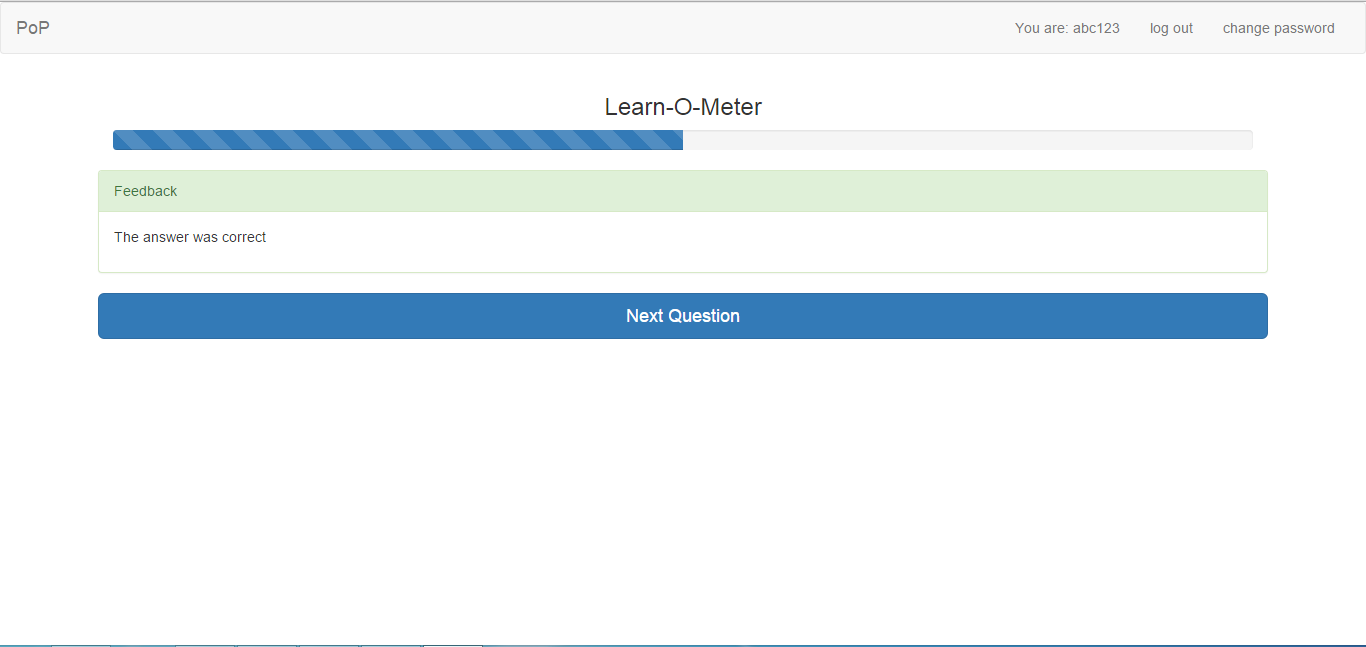
\includegraphics[width=1\linewidth]{figures/interface/answer.png}
    \caption{Screenshot af svar-siden.}
    \label{fig:screenshot_answer}
\end{figure}

\FloatBarrier

\subsubsection{Admin}
\label{subsub:screenshots_admin}
Når man er logget ind som administrator dukker der to nye links op i navigationsbaren ude på forsiden. Det første hedder \emph{admin}, og tager en til admin index-siden, som kan ses på Figur \ref{fig:screenshot_admin_home}. Her kan man se at der er kommet en ny navigationsbar, som giver adgang til diverse admin sider. \emph{Overview} tager en tilbage til forsiden.

\begin{figure}[htpb]
    \centering
    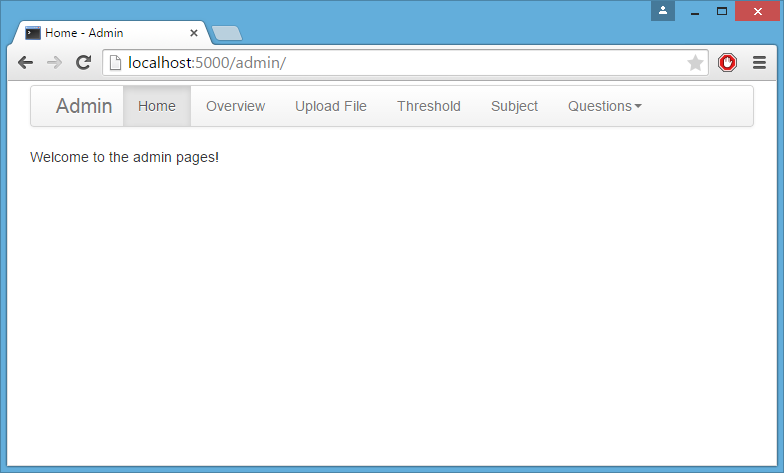
\includegraphics[width=1\linewidth]{figures/interface/admin_home.png}
    \caption{Screenshot af administratorernes index-side.}
    \label{fig:screenshot_admin_home}
\end{figure}

Den første af disse er \emph{Upload File}, som tager en til den side der kan ses på Figur \ref{fig:screenshot_admin_upload}. Her kan man uploade en YAML fil, og hvis den er korrekt udfyldt bliver der så oprettet et nyt spørgsmål i databasen.

\begin{figure}[htpb]
    \centering
    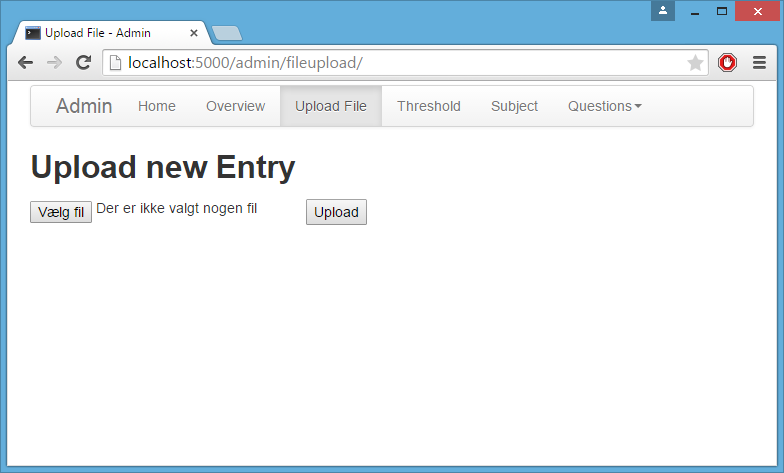
\includegraphics[width=1\linewidth]{figures/interface/admin_upload.png}
    \caption{Screenshot af administratorernes upload-side.}
    \label{fig:screenshot_admin_upload}
\end{figure}

Størstedelen af de andre links tager en til sider hvor man kan få et overblik over databasen. På Figur \ref{fig:screenshot_admin_subject} kan man se \emph{subject} siden, hvor man kan få et overblik over de \emph{subject} der er i databasen og deres diverse attributter. Det er desuden muligt at ændre på disse ved at trykke på blyant-knappen i venstre side af hver række, samt at slette \emph{subjects} ved at trykke på skraldespands-knappen.

\begin{figure}[htpb]
    \centering
    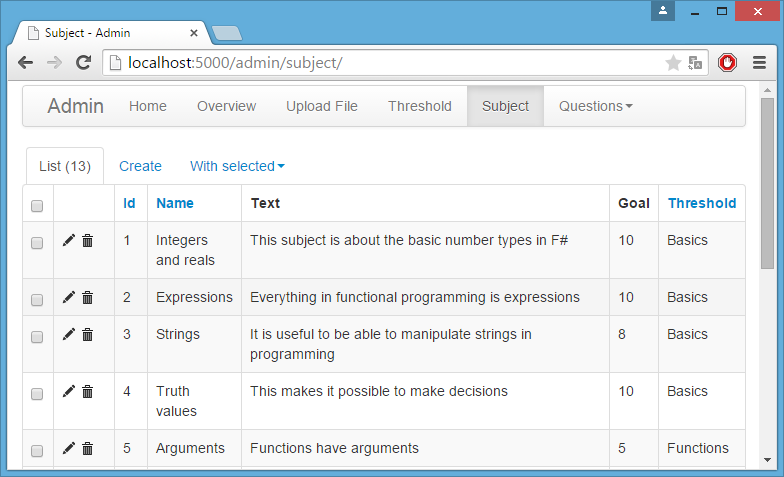
\includegraphics[width=1\linewidth]{figures/interface/admin_subject.png}
    \caption{Screenshot af administratorernes \emph{subject}-side.}
    \label{fig:screenshot_admin_subject}
\end{figure}

Hvis man i navigationsbaren trykker på \emph{Question} åbner man en dropdown menu, hvor man så kan vælge blandt de forskellige typer af spørgsmål i databsen og deres tilhørende svarmuligheds-objekter. På Figur \ref{fig:screenshot_admin_question} kan man f.eks. se de generelle spørgsmål objekter.

\begin{figure}[htpb]
    \centering
    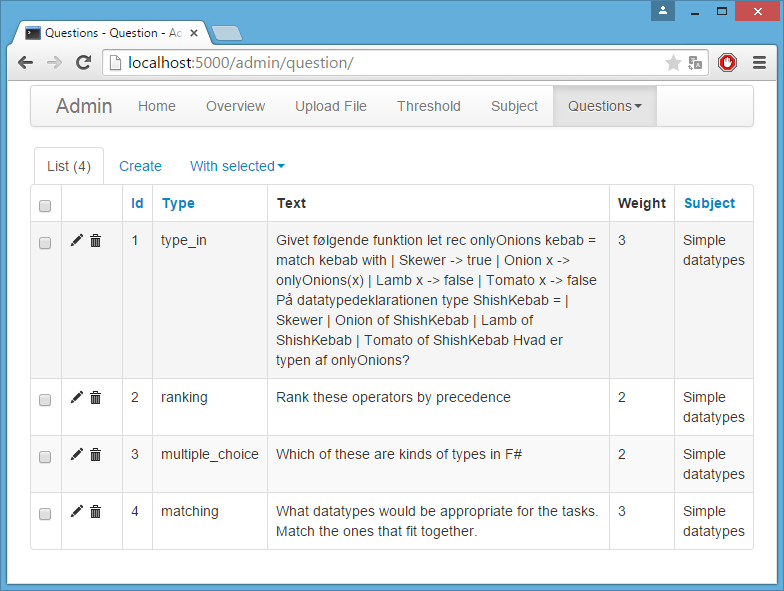
\includegraphics[width=1\linewidth]{figures/interface/admin_question.png}
    \caption{Screenshot af administratorernes spørgsmål-side.}
    \label{fig:screenshot_admin_question}
\end{figure}

Det andet nye link på forsiden er \emph{Log}, der tager en til log-siden der kan ses på Figur \ref{fig:screenshot_admin_log}. Herfra kan man se alle de forskellige informationer der bliver gemt hver eneste gang en bruger besvarer et spørgsmål.

\begin{figure}[htpb]
    \centering
    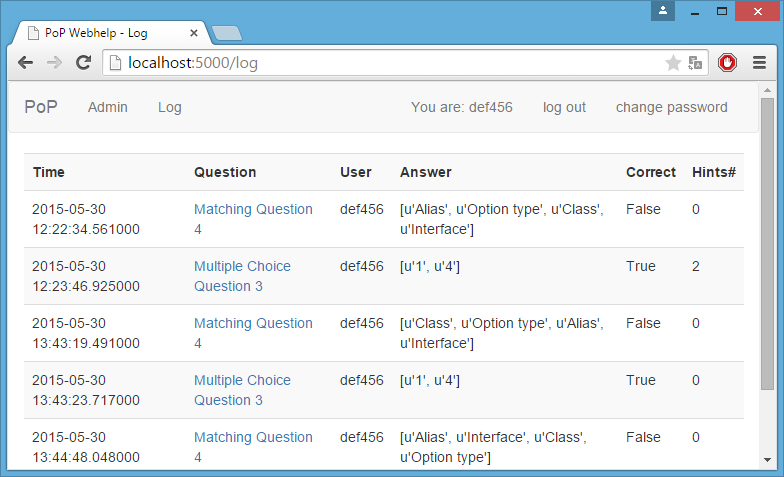
\includegraphics[width=1\linewidth]{figures/interface/admin_log.png}
    \caption{Screenshot af administratorernes log-side.}
    \label{fig:screenshot_admin_log}
\end{figure}

\FloatBarrier

\subsection{Flow-diagrammer}
\label{sub:flow_charts}
På Figur \ref{fig:flow_chart_login} ses en illustration af flowet i de forskellige handlinger man kan foretage sig ifb. med login-systemet. De forskellige pile antager at man indtaster de korrekte oplysninger og at der ikke sker nogle fejl, fordi hvis man f.eks. prøver at logge ind med et forkert kodeord lykkes det naturligvis ikke, og man kan selvfølgelig ikke registrere en ny bruger med et KU-id der allerede er brugt.

\begin{figure}[htpb]
    \centering
    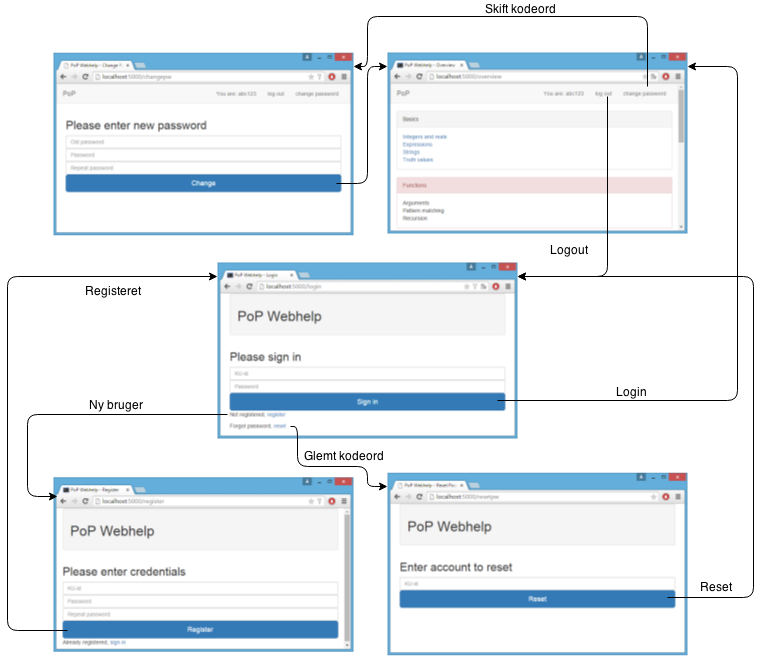
\includegraphics[width=1\linewidth]{figures/interface/flow_login.png}
    \caption{Flowchart over login-grænsefladen.}
    \label{fig:flow_chart_login}
\end{figure}
\FloatBarrier

På Figur \ref{fig:flow_chart_student} ses en illustration af flowet i en almindelig studerende interaktion med hjemmesiden, specifikt for når den studerende besvarer spørgsmål inden for et bestemt \emph{subject}.

\begin{figure}[htpb]
    \centering
    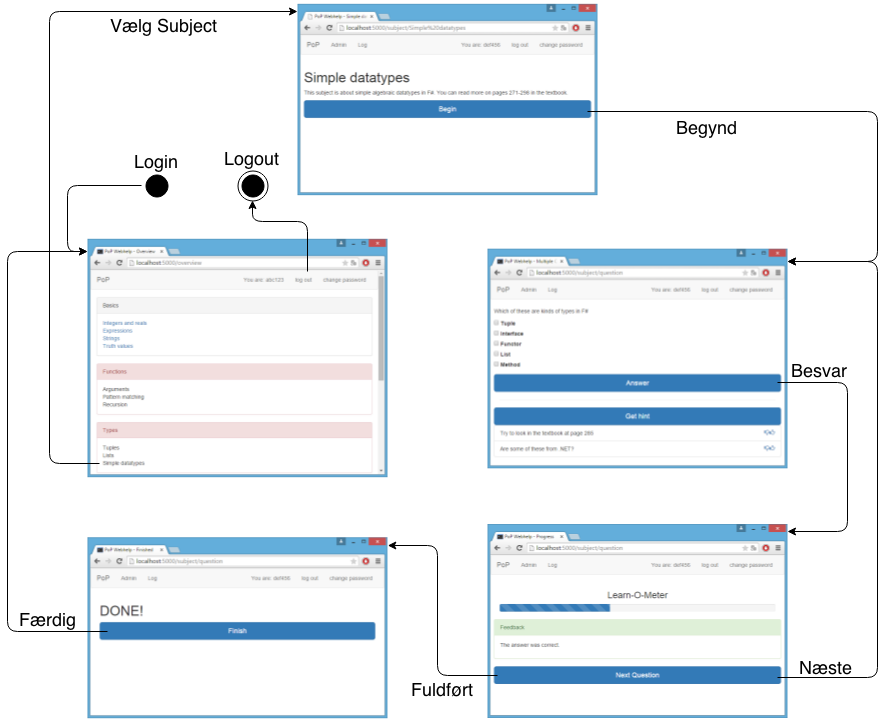
\includegraphics[width=1\linewidth]{figures/interface/flow_student.png}
    \caption{Flowchart over de studerendes brugergrænseflade.}
    \label{fig:flow_chart_student}
\end{figure}
\FloatBarrier

På Figur \ref{fig:flow_chart_admin} ses en illustration af flowet i en admins interaktion med hjemmesiden.

\begin{figure}[htpb]
    \centering
    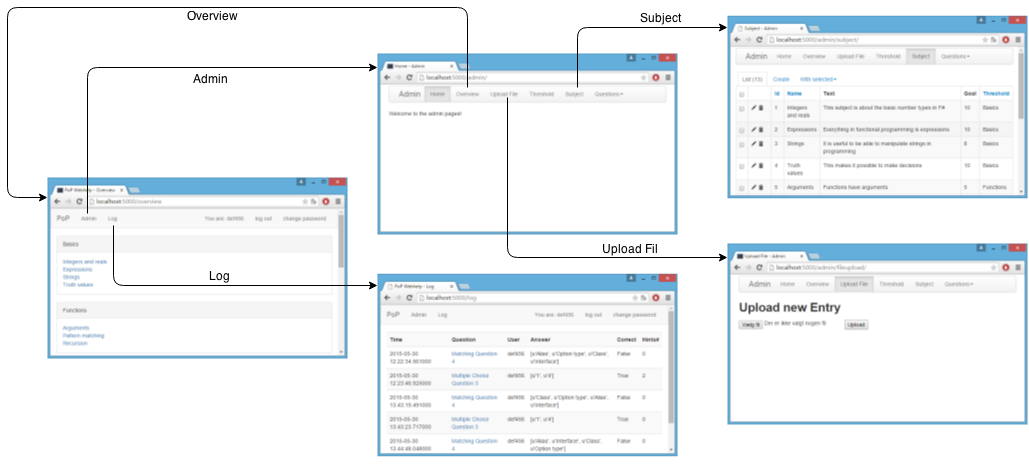
\includegraphics[width=1\linewidth]{figures/interface/flow_admin.png}
    \caption{Flowchart over admin brugergrænsefladen.}
    \label{fig:flow_chart_admin}
\end{figure}
\FloatBarrier

\subsection{AV-præsentation}
\label{sub:av_praesentation}

Der kan ses en præsentation af de vigtigste elementer i systemet på
\begin{framed}
    \centering
    \url{https://youtu.be/JexAhDF9XCc}
\end{framed}
Den viser hovedfunktionaliteten af systemet. Mere specifikt
\begin{itemize}
    \item Registrering som bruger.
    \item Besvarelse af opgaver.
    \item Navigering i admin delen.
\end{itemize}

\subsection{Tænke-højt forsøg}
\label{sub:taenke_hoejt}
Vi har udført \emph{tænke-højt} afprøvning af vores seneste prototype med en mulig bruger for vores system. Vi har ved denne test bedt en testperson om at løse en række opgaver på hjemmesiden som det beskrives i kapitel 9 i \cite{molich}. Mere specifikt er vedkommende blevet bedt om at logge ind, og derefter besvare et spørgsmål til et par emner. Ved denne afprøvning har vi identificeret en række problemer ved vores nuværende prototype, som skal addresseres i næste iteration af systemet. Som udgangpunkt lykkedes alle opgaverne uden hjælp, og derfor finder vi flowet af applikationen i orden.

Det vi skal have rettet er, at der skal være mere forklarende tekst til funktionaliteten på hjemmesiden. Det skal også fremgå mere tydeligt, hvor man skal indtaste sit svar, og det skal beskrives præcist, hvad der skal ske, når man er færdig med en opgave.

Mange af disse problemer er ikke ting vi har haft så meget fokus på under udviklingen, da vi har været mest interesserede i at få flowet på hjemmesiden til at være optimalt. Nu har vi observeret nogle enkelte problemer ved et \emph{tænke-højt forsøg}, og vi har planer om at rette det i næste iteration af systemet.

\section{Projektsamarbejdet}
\label{sec:projektsamarbejdet}
Samarbejdet med kunden er gået ganske udemærket. Når vi har mødtes med dem har der været en meget afslappet og munter stemning, og det harvirket som om vi har været meget godt på bølgelængde sammen og forstået at diskutere og blive enige om de forskellige aspekter af projektet. Vi har ikke været så gode til at være meget officielle og tage referater og notere alting ned, nok mest fordi møderne mere har været en mundtlig samtale og diskussion af projektet, hvor det er blevet tegnet både på papir og tavler. De ting vi er blevet enige om har desuden sjældent været helt nye for os, men nærmere været ting vi allerede selv havde ting over, og derfor har vi ikke følt at det har været nødvendigt at notere noget ned. Vi har først ved sidste møde haft en fungerende prototype at vise frem, men den virkede de til gengæld også imponerede over.

Projektsamarbejdet internt i gruppen er gået nogenlunde, her har vi heller ikke været så gode til at holde officielle møder  med dagsordener og referater og lignende. I stedet har vi mere bare snakket sammen når vi lige er mødtes inde på universitetet, og vi har primært arbejdet på projektet når vi lige har tid, f.eks. når vi har haft en pause eller en fri eftermiddag. Det meste af vores kommunikation både indbyrdes og med kunden er foregået over email.

Vi har forholdsvis sent i projektet fået oprettet en to-do liste inde i vores git repository, hvor vi har prøvet at notere de forskellige opgaver der manglede at blive løst ned, og som vi løbende har opdateret når vi har fået gennemført nogle af tingene eller er stødt på nye ting der skal laves, og det har fungeret rigtig godt. Det har hjulpet os til at have et bedre overblik over projektet, og til at ikke glemme alle de små ting man kan støde på og tænke at man løser senere.

\newpage
\appendix
\section{Versionsstyring}
\label{sec:versionsstyring}
Link til github: \url{https://github.com/christiankjaer/pop-webhelp}

\subsection{Git log}
\label{sub:git_log}

\VerbatimInput[fontsize=\tiny]{git-log.txt}

\section{Changelog}
\label{sec:changelog}
\begin{tabular}{p{0.15\textwidth} p{0.1\textwidth} p{0.75\textwidth}}
08-04-2015 & CKL & Dokument oprettet. \\
14-04-2015 & CKL & Tilføjet use cases og krav. \\
16-04-2015 & LSE & Tilføjet UseCaseModel og BCE model. \\
16-04-2015 & CKL & Tilføjet review af Parnas og Clements. \\
17-04-2015 & TSH & Tilføjet review af Gould og Lewis. \\
17-04-2015 & LSE & Tilføjet Abstract og Projektsamarbejdet. \\
17-04-2015 & CKL & Tilføjet use cases, sekvensdiagram og klassediagram. \\
26-04-2015 & CKL & Tilføjet afsnit om tests. \\
30-04-2015 & CKL & Rettet til genaflevering og tilføjet systemdesign. \\
08-05-2015 & CKL & Tilføjet afsnit om strukturering. \\
10-05-2015 & LSE & Tilføjet Brugergrænseflade og screenshots. \\
11-05-2015 & CKL & Tilføjet review af \cite{nsbullet}. \\
20-05-2015 & CKL & Tilføjet afsnit omkring systemdesign af brugere og begyndt på spørgsmål. \\
30-05-2015 & LSE & Tilføjet flere screenshots og flow-charts. \\
31-05-2015 & LSE & Tilføjet review af Naur. \\
01-06-2015 & CKL & Tilføjet integrationstestafsnit og TH-forsøg. \\
\end{tabular}

\section{Timeline}
\label{sec:timeline}
\begin{tabular}{p{0.15\textwidth} p{0.35\textwidth} p{0.5\textwidth}}
11-03-2015 & Første møde med kunde: & Vi har første møde med kunden hvor vi snakker om hvad projektet går ud på og diskuterer krav og løsningsforslag. \\
16-04-2015 & Andet møde med kunde: & Vi har haft andet møde med kunden, hvor vi har snakket om modellen for de opgaver der skal være i systemet. \\
22-04-2015 & Internt møde i gruppen: & Vi har diskuteret databasemodeller, og vi er kommet frem til et databaseskema for denne iteration af systemet. Derudover fik vi udviklet i fællesskab på systemet. \\
27-04-2015 & Tredje møde med kunde: & Vi blev enige om en endelig funktionalitet for den første iteration af produktet. Derudover diskuterede vi udformingen af spørgmsålstyper og hvordan det hele skulle knyttes sammen. \\
07-05-2015 & Internt møde i gruppen: & Vi mødtes internt i gruppen for at diskutere udestående implementationsopgaver, og kigge på nogle ting sammen. \\
07-05-2015 & Første fungerende prototype: & Vores første fungerende prototype af vores projekt er færdig, hvor vi har fået bundet alle de elementer vi løbende har lavet sammen til et sammenhængende hele. Admin aspektet mangler stadig. \\
21-05-2015 & Endelige protype færdig: & Vi har færdiggjort vores endelige prototype med alle de store elementer på plads. \\
27-05-2015 & Afsluttende møde med kunde: & Vi havde vores endelige møde med kunden hvor vi præsenterede dem for vores seneste prototype. Kunden virkede imponeret, og vi diskuterede mulighederne for at arbejde videre på projektet. \\
01-06-2015 & Usability test: & Vi har udført en usability test med kunden Martin, hvor vi har ladet ham prøve at bruge vores system, samtidig med at vi har stået på sidenlinjen og kigget med og noteret hans forskellige kommentarer ned. \\ 
\end{tabular}

\newpage

\bibliographystyle{plain}
\bibliography{refs}{}

\end{document}
